\documentclass[conference,letterpaper]{IEEEtran}

\usepackage[T1]{fontenc}
\usepackage[utf8]{inputenc}
\usepackage{mathptmx}
\usepackage[spanish,es-tabla,es-nodecimaldot,es-noshorthands]{babel}
\usepackage{icomma}
\usepackage{microtype}
\usepackage{amsmath,amssymb}
\usepackage{graphicx}
\usepackage{booktabs}
\usepackage{array}
\usepackage{multirow}
\usepackage{url}
\usepackage[hidelinks]{hyperref}

\renewcommand{\figurename}{Fig.}
\renewcommand{\tablename}{Tabla}
\renewcommand{\refname}{REFERENCIAS}

\title{Sistema de Alertas clínicas tempranas con IA interpretable para la predicción de riesgos en niños prematuros y de bajo peso del Programa Madre Canguro}

\author{
\IEEEauthorblockN{
Alex Paul Chirino Caicedo,
Breitner Enrique González,
Santiago José Ramos Echeverry,
Wilfrido Alberto Gómez Pérez
}
\IEEEauthorblockA{
Universidad de los Andes -- Fundación Canguro\\
Maestría en Inteligencia Artificial, Octubre de 2026
}
}

\begin{document}
\maketitle

\section{Descripción breve de la propuesta de solución}

Se desarrolló una solución de inteligencia artificial (IA) interpretable para apoyar la revisión de registros longitudinales y la estimación de riesgos en niños prematuros o de bajo peso vinculados al Programa Madre Canguro. La propuesta responde a dos dificultades complementarias: la calidad variable de los registros clínicos y la necesidad de anticipar desenlaces antes de la siguiente visita. El sistema no emite diagnósticos ni reemplaza la valoración profesional: organiza datos, identifica observaciones dudosas y produce estimaciones probabilísticas con explicaciones.

La solución consta de dos modelos encadenados. El primero examina la conformidad y plausibilidad de los datos mediante reglas, modelos contextuales y comparaciones longitudinales; el segundo utiliza información disponible hasta un corte de seguimiento para estimar riesgos clínicos por desenlace. El umbral que transforma un riesgo en una notificación pertenece a la aplicación y a la gobernanza clínica, no al entrenamiento del clasificador. El enfoque permite separar errores de captura de señales potencialmente clínicas y mantener trazabilidad de las decisiones.

El alcance se ajustó al comportamiento real de la fuente: en lugar de reentrenamiento mensual y escritura de resultados en la base institucional, se adoptó una corrida alineada con la carga semestral, manteniendo inferencia a demanda y separación entre datos reales y simulados. Esta decisión reduce dependencias operativas y permite evaluar el sistema con cortes reproducibles.

La solución se despliega como servicio con registro de modelos, API de inferencia y tablero web, en un entorno público con datos simulados y uno interno con datos reales. Se discuten sus aplicaciones para priorizar el seguimiento clínico y sus límites: pérdida de seguimiento y deriva de calibración.

\begin{figure}[!t]
    \centering
    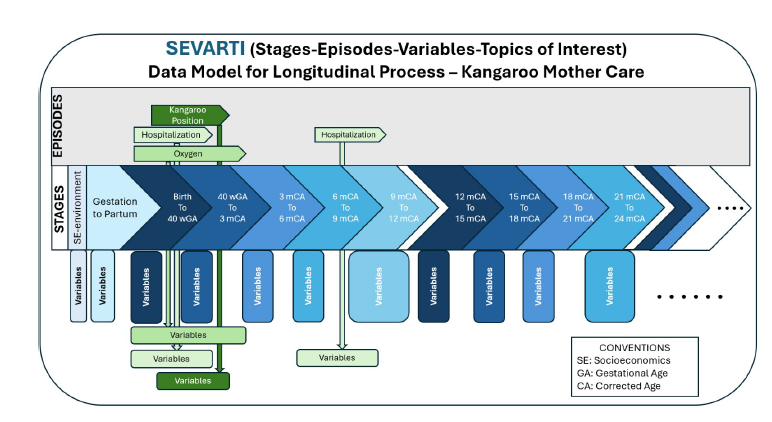
\includegraphics[width=\columnwidth]{figuras/figura1_sevarti.png}
    \caption{Modelo conceptual SEVARTI: etapas, episodios y variables.}
    \label{fig:sevarti}
\end{figure}

\section{Recolección y preparación de los datos}

\subsection{Fuente, extracción y contrato de datos}

SEVARTI (\textit{Stages--Episodes--Variables--Topics of Interest}) organiza procesos longitudinales mediante etapas de desarrollo, episodios de atención y variables vinculadas a cada momento. En el Programa Madre Canguro permite ubicar los controles y antecedentes sobre un eje de edad gestacional o corregida, diferenciando visitas programadas de episodios con duración propia.

Se emplearon registros de la capa de consumo de una base PostgreSQL institucional, consultada con permisos de solo lectura. El corte documentado corresponde al 24 de julio de 2026. Los informes técnicos del equipo registran 62.043 pacientes y aproximadamente 13,9 millones de mediciones; estas cifras describen el universo de datos del corte y no el número efectivo de observaciones de cada modelo. La extracción incorpora datos perinatales, controles antropométricos, visitas, eventos clínicos y episodios de atención.

El adaptador SEVARTI representa la información mediante seis entidades: esquema, etapas, sujetos, mediciones, episodios y quiebres históricos. Un diccionario administrado por expertos define variables, unidades, conceptos longitudinales, códigos de ausencia, ventanas de visita y desenlaces. Las versiones de documentación presentan diferencias en el número de variables (339--342), por lo que el conteo definitivo debe acompañarse del identificador del diccionario utilizado en cada experimento.

El corte principal reúne 62.043 niños, 13.884.056 mediciones y 339 variables catalogadas (318 en uso), según la versión documentada del artículo en desarrollo. Las cifras deben asociarse siempre al corte y al criterio de conteo, pues versiones anteriores contenían 15.641 niños y aproximadamente 4,5 millones de mediciones. El 76\,\% de los registros carece de ubicación temporal explícita, por lo que el adaptador reconstruye el contexto con la etapa, la edad anotada y las fechas verificables.

La partición experimental se efectuó por niño y año de nacimiento, con separación de los regímenes anteriores y posteriores al cambio de registro de 2022. Para anomalías se reportaron 40.711 niños en entrenamiento, 7.330 en calibración y 8.955 en prueba; para clasificación clínica, 48.041 en entrenamiento y 8.955 en prueba. Estas cantidades pertenecen a configuraciones experimentales distintas y no deben sumarse como si constituyeran un único particionamiento.

\subsection{Edad corregida, consistencia y tratamiento de faltantes}

La edad corregida en días se obtuvo como
\begin{equation}
EC=\text{edad posnatal (días)}-7(40-\text{edad gestacional en semanas}).
\end{equation}

Se contrastaron fechas de nacimiento y visitas, edades consignadas, orden temporal y ventanas de seguimiento. Para el análisis de crecimiento se conservaron las edades reales de medición, dado que diferencias de semanas pueden afectar la interpretación del peso, talla y perímetro cefálico. Los valores dudosos se etiquetan para revisión y, según el protocolo del modelo, se excluyen como valores válidos o se tratan como faltantes; no se sustituyen automáticamente por valores estimados.

La auditoría identificó códigos de relleno no documentados en 14 variables, registros con unidades inconsistentes, fechas imposibles, medidas fuera de la ventana prevista y cambios de codificación alrededor de 2022. Se observó además pérdida de seguimiento: el registro de peso se aproxima al 78\,\% en 40 semanas y al 49\,\% a los 12 meses de edad corregida. Esta caída exige distinguir entre ausencia de dato, ausencia de visita y pérdida de seguimiento, pues la cohorte de casos completos puede no representar a todos los niños.

\begin{figure}[!t]
    \centering
    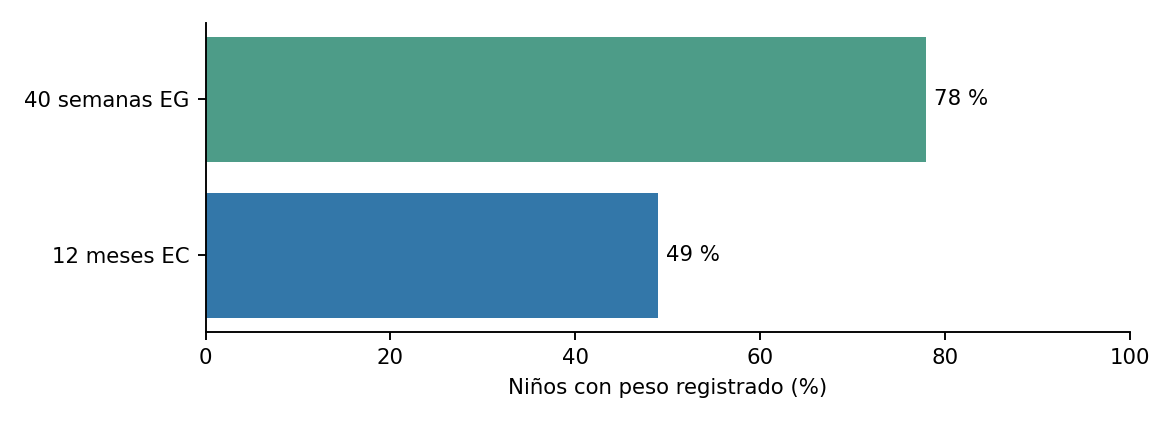
\includegraphics[width=\columnwidth]{figuras/figura2_cobertura_peso.png}
    \caption{Cobertura de peso en dos controles, según auditoría interna del corte 24/07/2026.}
    \label{fig:cobertura}
\end{figure}

\section{Descripción del proceso de construcción de los modelos o solución}

\subsection{Flujo reproducible y control de versiones}

La ejecución se organiza en preparación SEVARTI, validación del diccionario, detección de anomalías, construcción de variables clínicas, entrenamiento por desenlace, evaluación y cálculo de riesgos. Cada actualización institucional puede iniciar una nueva corrida; el pipeline contempla una modalidad de evaluación silenciosa, en la cual los riesgos se guardan antes de conocer los desenlaces posteriores. Los resultados, modelos y artefactos se versionan para conservar reproducibilidad y permitir comparaciones entre cortes.

La trazabilidad del entrenamiento depende de una máscara de exclusiones versionada: se conservan los datos originales, mientras los códigos especiales, errores de unidad y extremos claramente inconsistentes se excluyen como objetivos de entrenamiento y se representan como faltantes en los modelos posteriores. La documentación del corte registra una exclusión del 1,6\,\% de aproximadamente 3,53 millones de datos numéricos; ello no equivale a eliminar pacientes completos.

\subsection{Modelo de anomalías: cinco niveles de revisión}

Una anomalía es una observación que incumple el contrato de registro o resulta improbable por su valor, contexto clínico, trayectoria o periodo. No constituye necesariamente un error confirmado ni un diagnóstico: indica que el dato requiere revisión. Un peso plausible aisladamente, por ejemplo, puede ser incompatible con la edad corregida o con mediciones anteriores.

La revisión robusta calcula
\begin{equation}
z_r=\frac{x-\mathrm{mediana}}{1.4826\,\mathrm{MAD}},
\end{equation}
con MAD como mediana de desviaciones absolutas, y señala candidatos cuando $|z_r|>3.5$.

La capa contextual estima $Q_{0.25}$, $Q_{0.50}$ y $Q_{0.75}$; el residuo
\begin{equation}
z_2=\frac{y-Q_{0.50}}{(Q_{0.75}-Q_{0.25})/1.349}
\end{equation}
se contrasta con un umbral conformal obtenido del cuantil $1-\alpha$ de $|z_2|$ en calibración, con $\alpha=0.005$.

\begin{table}[!t]
\caption{Niveles de revisión de anomalías}
\label{tab:anomalias}
\centering
\scriptsize
\begin{tabular}{p{0.13\columnwidth} p{0.33\columnwidth} p{0.41\columnwidth}}
\toprule
Nivel & Procedimiento & Salida o propósito \\
\midrule
0. Contrato & Tipo, unidad, códigos y ubicación temporal & Dato válido, rechazado o no ubicable \\
1. Valor & Estadísticos robustos, extremos y escala & Valores anómalos o errores de unidad \\
2. Contexto & LightGBM cuantílico y residuo calibrado & Incompatibilidad con antecedentes y visita \\
3. Trayectoria & Diferencias y velocidades entre medidas & Saltos inesperados y secuencias incoherentes \\
4. Grupo-tiempo & Cambios trimestrales, redondeo y faltantes & Cambios en prácticas de registro \\
\bottomrule
\end{tabular}
\end{table}

En la capa contextual se estiman cuantiles condicionales de cada variable a partir de otras características del niño, la visita y el momento de medición, excluyendo el propio valor evaluado. La metodología utiliza un criterio de calibración de residuos y, cuando hay suficiente muestra, un umbral de alerta de $p\leq0.005$.

La capa longitudinal contrasta cambios entre visitas con velocidades de referencia y tolerancias por concepto; la capa temporal busca alteraciones sistemáticas en grupos o periodos. La salida prioriza registros para revisión y proporciona motivos, no una etiqueta clínica definitiva.

Se ajustaron tres regresiones cuantílicas por variable numérica. La vigilancia temporal agrega indicadores trimestrales de residuos, faltantes y redondeo, contrastados con los ocho trimestres previos y analizados mediante CUSUM. El entrenamiento documentado generó 132 modelos contextuales en 15,7 minutos de CPU.

\subsection{Clasificación de riesgos y explicabilidad}

Para cada desenlace y corte de seguimiento se preparan firmas con antecedentes basales, historia de visitas, episodios y mediciones conocidas hasta ese instante. Los clasificadores LightGBM estiman probabilidades que se calibran y se comparan con reglas simples. Las explicaciones basadas en TreeSHAP permiten examinar contribuciones de variables a una predicción, sin atribuirles interpretación causal. Las particiones por paciente y la separación cronológica son indispensables para evitar que información de controles futuros contamine la validación.

La documentación registra 14 desenlaces evaluados, incluyendo readmisión, inasistencia a la siguiente visita, oxigenodependencia, desarrollo y resultados de crecimiento. Para cada uno se deben fijar de manera explícita la fecha índice, horizonte de predicción, definición de etiqueta y criterios de elegibilidad.

Los 14 desenlaces modelados incluyen cinco ventanas de readmisión, cinco de ausencia a la siguiente visita, dos evaluaciones de oxigenodependencia y dos de desarrollo psicomotor bajo. Los cuatro desenlaces adicionales de crecimiento a 12 meses se consideran una extensión diferenciada y no deben contarse como parte de los 14 modelos ya evaluados.

Para disminuir fuga de información, las características se restringen a los registros disponibles hasta cada visita; se descartan variables completadas retrospectivamente y los casos de inasistencia solo se etiquetan una vez cerrada la ventana de seguimiento. Las probabilidades se calibran mediante regresión isotónica con una partición temporal posterior al entrenamiento; la salida incluye riesgo, percentil y contribuciones locales TreeSHAP.

\subsection{Trayectorias antropométricas y firmas incrementales}

Una trayectoria antropométrica es la sucesión ordenada de peso, talla y perímetro cefálico de un niño, con sus edades reales y eventos asociados. Su análisis incluye nivel, dirección, velocidad y cambios de pendiente, preferiblemente mediante puntajes $z$ de una referencia adecuada a sexo y edad corregida.

Se estableció una trayectoria de ocho hitos: nacimiento, inicio de posición canguro, salida de posición canguro, 40 semanas de edad gestacional y controles de 3, 6, 9 y 12 meses de edad corregida. Los dos hitos de posición canguro se interpretan como eventos con fecha propia y no como visitas a una edad fija.

Para predecir un desenlace a 12 meses se proyectan firmas sucesivas en 40 semanas, 3, 6 y 9 meses. Cada firma puede incluir estado actual, cambio respecto al control anterior, velocidad por día, trayectoria histórica, variables basales y señales de calidad. La selección de variables combina plausibilidad clínica, disponibilidad antes del corte, completitud, estabilidad temporal y ganancia predictiva frente a una línea base.

\begin{table}[!t]
\caption{Firmas incrementales propuestas}
\centering
\scriptsize
\begin{tabular}{p{0.20\columnwidth} p{0.47\columnwidth} p{0.23\columnwidth}}
\toprule
Corte & Información admisible & Desenlace \\
\midrule
40 semanas & Nacimiento, episodios neonatales y datos hasta 40 semanas & Estado a 12 meses EC \\
3 meses EC & Firma previa + mediciones y eventos hasta 3 meses & Estado a 12 meses EC \\
6 meses EC & Firma previa + cambios y eventos hasta 6 meses & Estado a 12 meses EC \\
9 meses EC & Firma previa + cambios y eventos hasta 9 meses & Estado a 12 meses EC \\
\bottomrule
\end{tabular}
\end{table}

La evaluación incremental propuesta distingue cuatro firmas predictivas y un desenlace a 12 meses. Las interpolaciones entre visitas solo se usarán en análisis descriptivos o cuando se pueda garantizar que no emplean observaciones futuras respecto al instante de predicción.

\subsection{Arquitectura técnica y protección de datos}

El procesamiento de datos reales se mantiene en un equipo local con GPU, con acceso a PostgreSQL institucional de solo lectura. El entorno de trabajo integra CLI de entrenamiento, MLflow para seguimiento experimental, MinIO para artefactos, PostgreSQL local, FastAPI para inferencia y React/nginx para visualización.

El entorno de demostración en Railway utiliza únicamente datos simulados y un paquete de modelo destinado a ese propósito; no recibe historias clínicas reales. Las salidas individuales permanecen en el entorno autorizado.

La arquitectura contempla contenedores Docker para una ejecución semestral, un registro de experimentos y versiones en MLflow, artefactos en almacenamiento interno, inferencia mediante FastAPI y una interfaz React con funciones de administración, evaluación y visualización.

\begin{figure}[!t]
    \centering
    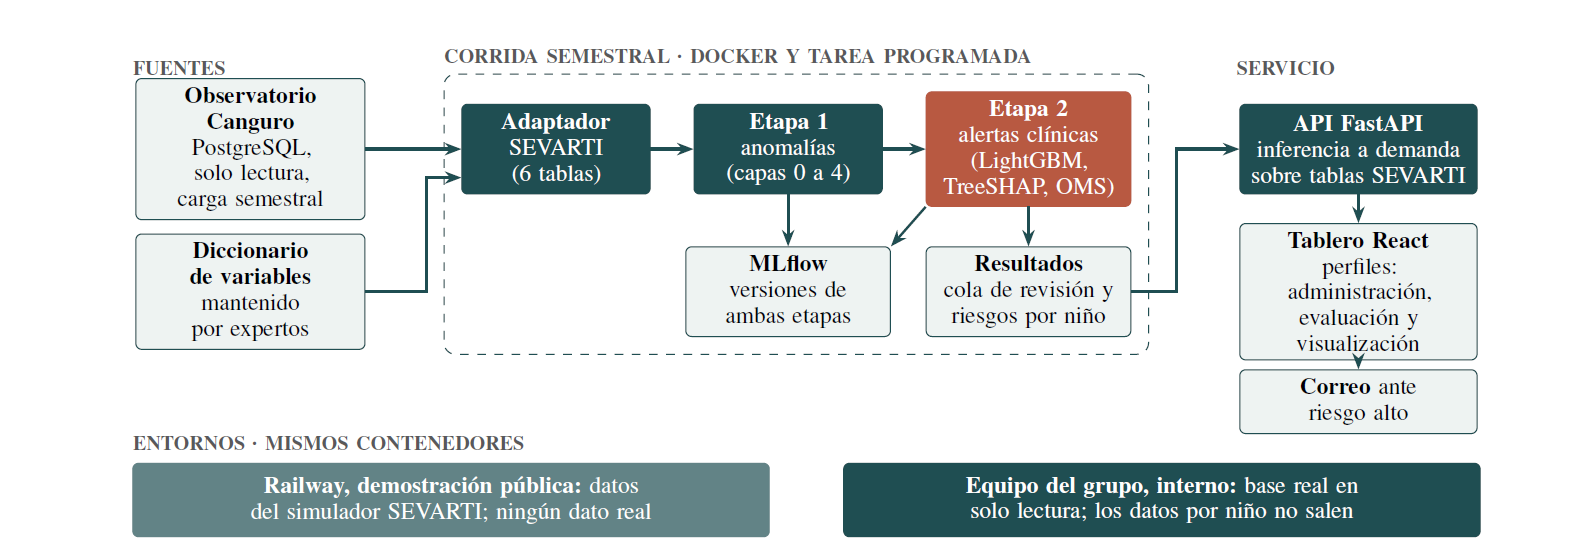
\includegraphics[width=\columnwidth]{figuras/figura3_arquitectura.png}
    \caption{Arquitectura lógica del sistema: SEVARTI, anomalías, riesgos y servicio.}
    \label{fig:arquitectura}
\end{figure}

\section{Resultados obtenidos}

La validación interna de los 14 desenlaces detalla el momento de cálculo, niños elegibles, prevalencia, AUC del modelo y de la regla simple, concentración de casos en el decil de mayor riesgo y razón riesgo medio/observado. Trece comparaciones de AUC favorecen al modelo. Para oxigenodependencia a tres meses se obtuvo AUC 0,91 frente a 0,80 de la regla, con 67,7\,\% frente a 49,3\,\% de los casos en el decil superior. La razón riesgo/observado de 1,58 indica sobreestimación y motiva recalibración.

\begin{figure*}[!t]
    \centering
    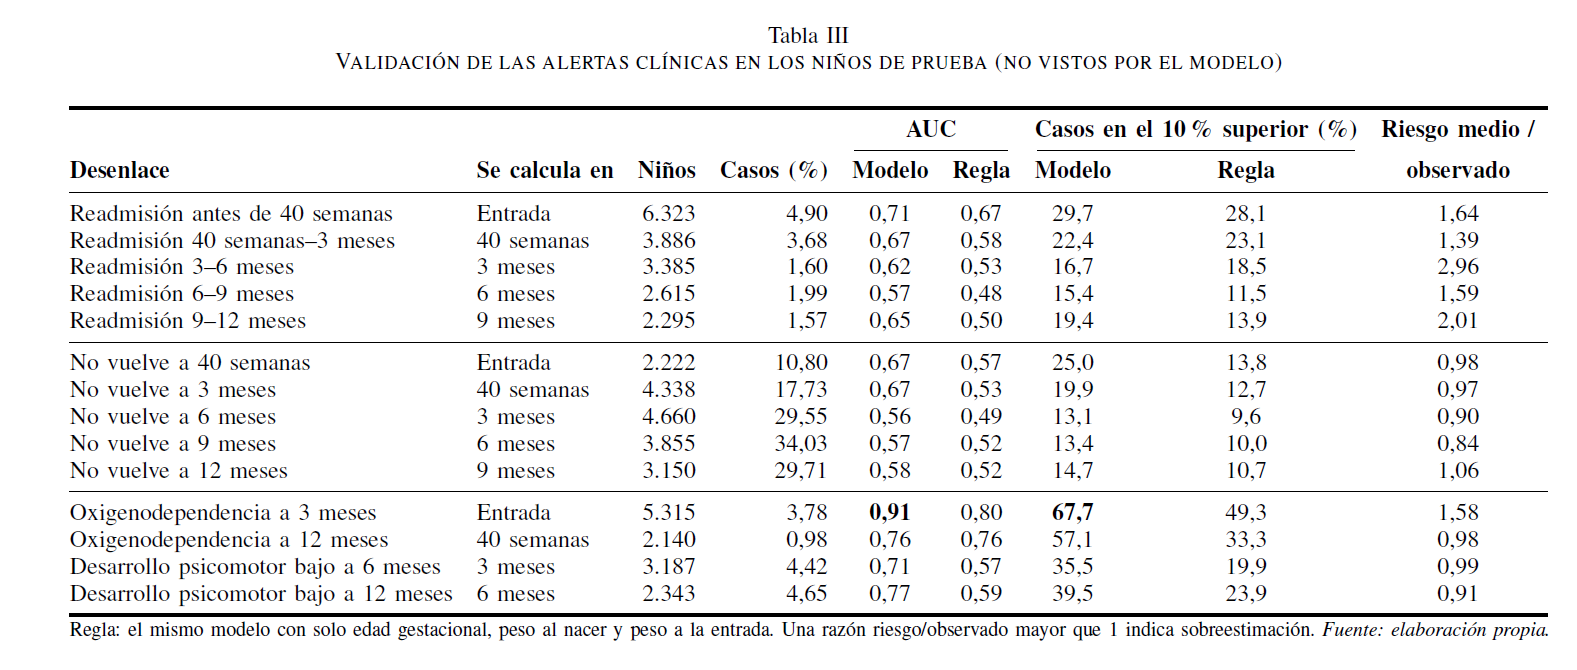
\includegraphics[width=0.92\textwidth]{figuras/tabla3_validacion.png}
    \caption{Validación retrospectiva por desenlace, corte 24/07/2026.}
    \label{fig:tabla3}
\end{figure*}

Los resultados corresponden a experimentos internos documentados para el corte analizado. No deben confundirse con una evaluación prospectiva definitiva, una validación externa o la aprobación clínica de las alertas.

El detector de anomalías mostró 78\,\% de detección de desvíos sintéticos de tres desviaciones estándar, frente a 27\,\% de una regla de rangos; también se reportó 68\,\% de detección de alteraciones de etapa. Estas cifras describen escenarios de prueba específicos y no la sensibilidad ante todos los errores reales.

\begin{figure}[!t]
    \centering
    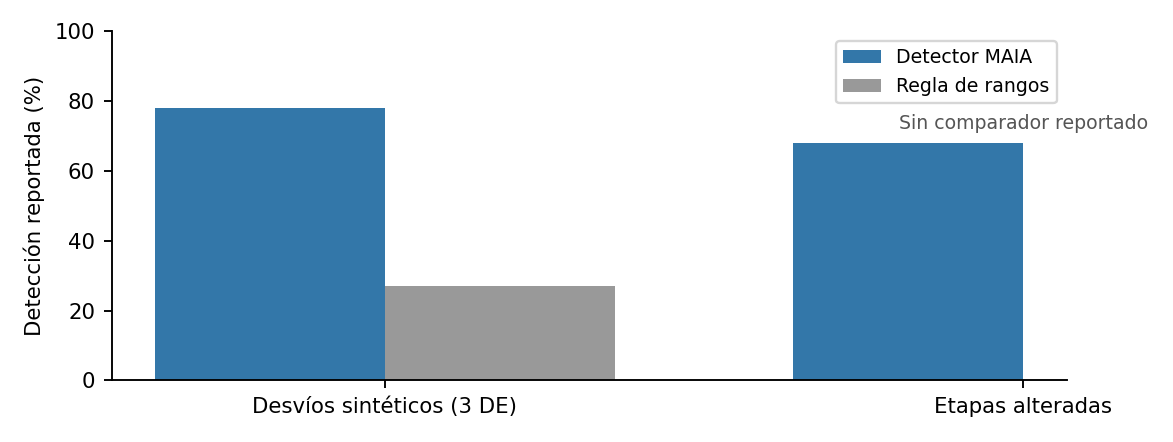
\includegraphics[width=\columnwidth]{figuras/figura4_anomalias.png}
    \caption{Detección en pruebas internas de perturbaciones sintéticas.}
    \label{fig:anomalias}
\end{figure}

Para oxigenodependencia a tres meses se reportó AUROC de 0,91. En el decil de mayor riesgo, el modelo concentró 67,7\,\% de los casos frente a 49,3\,\% con la referencia simple. Para desarrollo psicomotor relativamente bajo se documentaron AUROC de 0,71 a seis meses y 0,77 a doce meses.

\begin{figure}[!t]
    \centering
    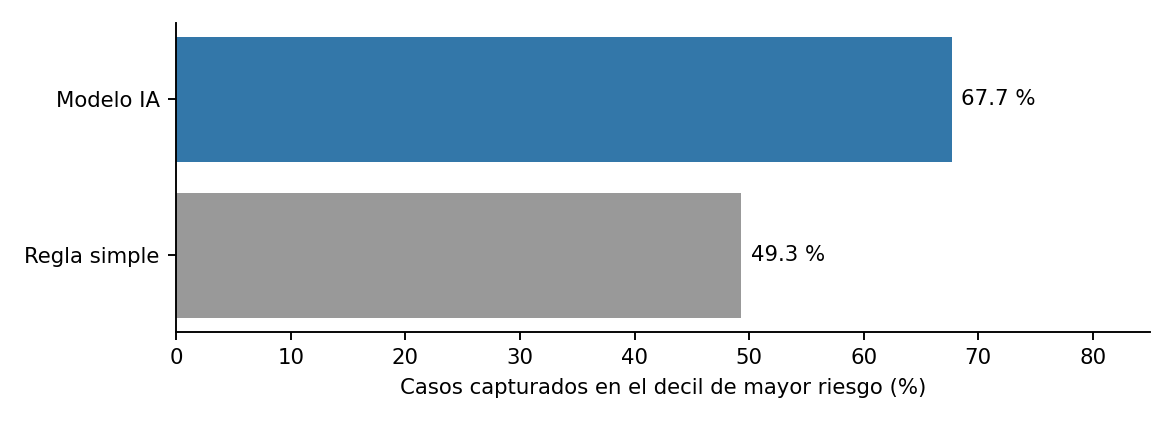
\includegraphics[width=\columnwidth]{figuras/figura5_oxigenodependencia.png}
    \caption{Concentración de casos de oxigenodependencia en el 10\,\% de niños con mayor riesgo.}
    \label{fig:oxigeno}
\end{figure}

En calidad de datos se identificaron 33 fechas imposibles, 985 eventos fechados antes del parto y 5.905 registros de crecimiento con edad distinta a la de la visita. Estos hallazgos apoyan el valor del control de calidad antes del modelamiento, pero requieren confirmación y depuración en origen.

La evaluación del detector inyectó seis clases de errores en la partición de prueba: códigos, unidades, desviaciones de tres desviaciones estándar, dígitos invertidos, intercambio de etapas y valores procedentes de otro niño. La detección global documentada fue del 75,3\,\% con 18,8 alertas por cada 1.000 registros sin perturbación inyectada, frente a 14,7 alertas de la regla vigente.

En el componente clínico, el artículo en desarrollo informa una AUROC entre 0,56 y 0,91 según desenlace, con mejora frente a la referencia simple en 13 de 14 comparaciones. Estas métricas describen discriminación en prueba retrospectiva; no equivalen a sensibilidad clínica en un umbral específico ni prueban utilidad prospectiva.

\section{Análisis de los resultados obtenidos, retos y cómo proseguir}

La lectura conjunta de AUC y calibración es esencial: un clasificador puede ordenar mejor el riesgo y simultáneamente sobreestimar probabilidades. Los desenlaces de inasistencia muestran discriminación moderada, con AUC de 0,56 a 0,67; se requiere evaluar por desenlace, con intervalos de confianza, precisión--recall y utilidad operativa, no solo mediante el número agregado de comparaciones favorables.

La mejora frente a reglas simples indica que el contexto del niño y su trayectoria contienen información útil que las verificaciones aisladas no capturan. No obstante, la evaluación con perturbaciones artificiales puede sobreestimar la detección de errores naturales. De manera análoga, un AUROC elevado no garantiza probabilidades bien calibradas ni una carga de alertas aceptable. La revisión humana y la evaluación de calibración por subgrupos son necesarias antes de cualquier uso asistencial.

La pérdida de seguimiento es un riesgo metodológico central. Exigir las 18 mediciones de peso, talla y perímetro cefálico en seis visitas generaría una cohorte altamente seleccionada; por ello, se reservará el subconjunto completo para análisis de sensibilidad, mientras que los clasificadores incrementales deben utilizar información disponible hasta cada corte y documentar patrones de ausencia.

Los cambios de captura alrededor de 2022 obligan a controlar quiebres históricos, verificar estabilidad de unidades y validar temporalmente en cohortes posteriores. También quedan por consolidar el diccionario de variables, las referencias de crecimiento según edad y población, la definición de algunos desenlaces y el manejo de mediciones registradas fuera de ventana.

Como continuación se propone: (i) congelar el corte y la versión del diccionario para reproducir métricas; (ii) completar auditoría por desenlace, curvas de calibración e intervalos de confianza; (iii) implementar y comparar firmas incrementales en 40 semanas, 3, 6 y 9 meses para predicción a 12 meses; (iv) revisar con expertos una muestra ciega de anomalías y alertas; y (v) contrastar las predicciones guardadas con un nuevo corte de la Fundación, cuando esté disponible, respetando el tiempo de maduración de cada desenlace.

La cobertura disminuye a medida que avanza el seguimiento: la documentación experimental registra alrededor de 78\,\% de peso disponible a las 40 semanas y 49\,\% a los 12 meses entre niños elegibles para cada visita. Por ello, la cohorte con las 18 mediciones completas debe utilizarse como análisis de sensibilidad y caracterización de trayectorias, no como único conjunto de entrenamiento.

El quiebre de registro de 2022 constituye una amenaza de deriva: los pesos redondeados a 100 g aumentaron del 0,9\,\% al 5,4\,\%, y las diferencias de prácticas de medición pueden confundirse con cambios biológicos. El aumento reportado de readmisiones desde 2021 también requiere contrastación con expertos de datos antes de atribuirlo a un cambio clínico real.

Finalmente, la incorporación de trayectorias incrementales se evaluará mediante una comparación controlada entre una línea base perinatal, un modelo con estado antropométrico actual y otro con cambios longitudinales acumulados. Solo la diferencia entre estos últimos permitirá cuantificar el aporte predictivo específico de la trayectoria. La explicación individual de los riesgos será sometida a revisión clínica y no se interpretará como evidencia causal.

\begin{thebibliography}{00}

\bibitem{villar2015}
J. Villar et al., ``Postnatal growth standards for preterm infants,'' \textit{The Lancet Global Health}, vol. 3, no. 11, pp. e681--e691, 2015, doi: 10.1016/S2214-109X(15)00163-1.

\bibitem{fenton2013}
T. R. Fenton and J. H. Kim, ``A systematic review and meta-analysis to revise the Fenton growth chart for preterm infants,'' \textit{BMC Pediatrics}, vol. 13, art. 59, 2013, doi: 10.1186/1471-2431-13-59.

\bibitem{tripod2024}
G. S. Collins et al., ``TRIPOD+AI statement: updated guidance for reporting clinical prediction models that use regression or machine learning methods,'' \textit{BMJ}, vol. 385, e078378, 2024, doi: 10.1136/bmj-2023-078378.

\bibitem{lightgbm2017}
G. Ke et al., ``LightGBM: A highly efficient gradient boosting decision tree,'' in \textit{Advances in Neural Information Processing Systems}, vol. 30, 2017.

\bibitem{shap2017}
S. M. Lundberg and S.-I. Lee, ``A unified approach to interpreting model predictions,'' in \textit{Advances in Neural Information Processing Systems}, vol. 30, 2017.

\bibitem{who2022}
World Health Organization, \textit{WHO Recommendations for Care of the Preterm or Low-Birth-Weight Infant}. Geneva, Switzerland: WHO, 2022.

\end{thebibliography}

\end{document}
\end{document}
